\section{Experimental set-up}
\begin{figure}[h]
\centering
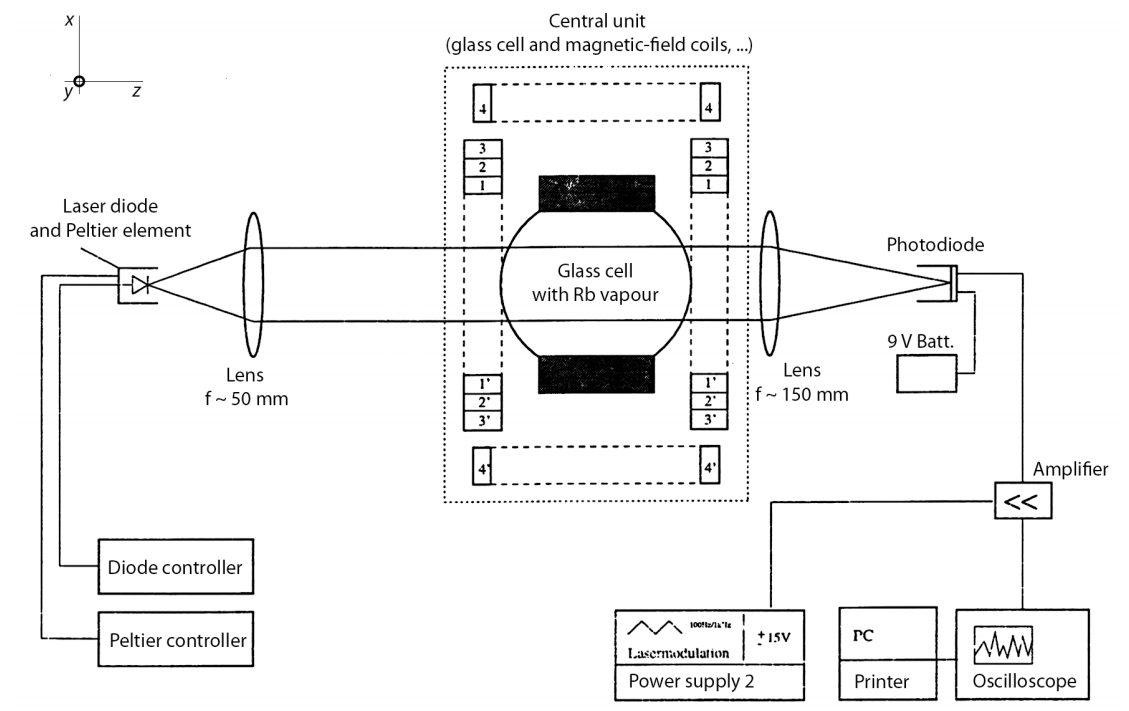
\includegraphics[width=1.0\linewidth]{graphics/generalsetup}
\caption[Basic experimental set-up]{Basic set-up of the experiment. For the various tasks, parts can be placed onto the optical bench. The glass cell can be removed from the central unit. \cite{anleitung} (modified)}
\label{fig:general setup}
\end{figure}
At the core of the experimental set-up is the glass cell with the Rubidium vapor and the buffer gas. It can be taken in and out of the central unit, which in turn houses four sets of Helmholtz coils. Another such pair is directly attached to the casing of the glass cell, along with a radio frequency generator and and appropriate frequency measuring device.\\

\textbf{A laser diode} provides coherent light in the energy range needed to pump the desired hyperfine state of the Rubidium atoms in the glass cell. Laser diodes send out linearly polarized light with a small spectral width. Frequency and intensity vary with the temperature of the diode as well as the current running through it, which is why the diode is kept at constant temperature using a Peltier element. For the diode to start emitting light, a certain current threshold has to be reached. From then on, the intensity depends linearly on the current if temperature is kept constant. However, mode jumps at certain currents disturb the linearity. Mode jumps occur when the number of standing waves in the resonator changes and measurements need to be taken in areas that do not include such jumps.\\

The beam is collimated by a lens before passing through other optical elements and, after passing through the central unit, is refocused onto a photo-diode. This can be seen in figure \ref{fig:general setup}. The output of the diode is amplified and can then be observed on an oscilloscope, which in turn can be read out by a computer to produce analyzable data.\\ 

The set-up varies greatly from one part of the experiment to another and will thus be explained in detail in the appropriate sections.

\
\section{Characterization of the laser diode}
For later measurements, it is important to determine the range of supply current in which the diodes intensity increases linearly without mode jumps occuring. The gas cell is taken out of the central unit for this part of the experiment. \\

After turning on the peltier element, a few minutes should pass before measurements are started to allow the diode to thermalize. Then, without any other parts being added to the optical path, the intensity of the diode is measured at supply currents between $\unit{0-90}{mA}$. The results can be seen in figure \ref{fig:characterization}. The threshold current is roughly $\unit{51.6}{mA}$, followed by the linear domain until mode jump occur at around $\unit{72}{mA}$ to $\unit{82}{mA}$. 
\begin{figure}[htb]
\centering
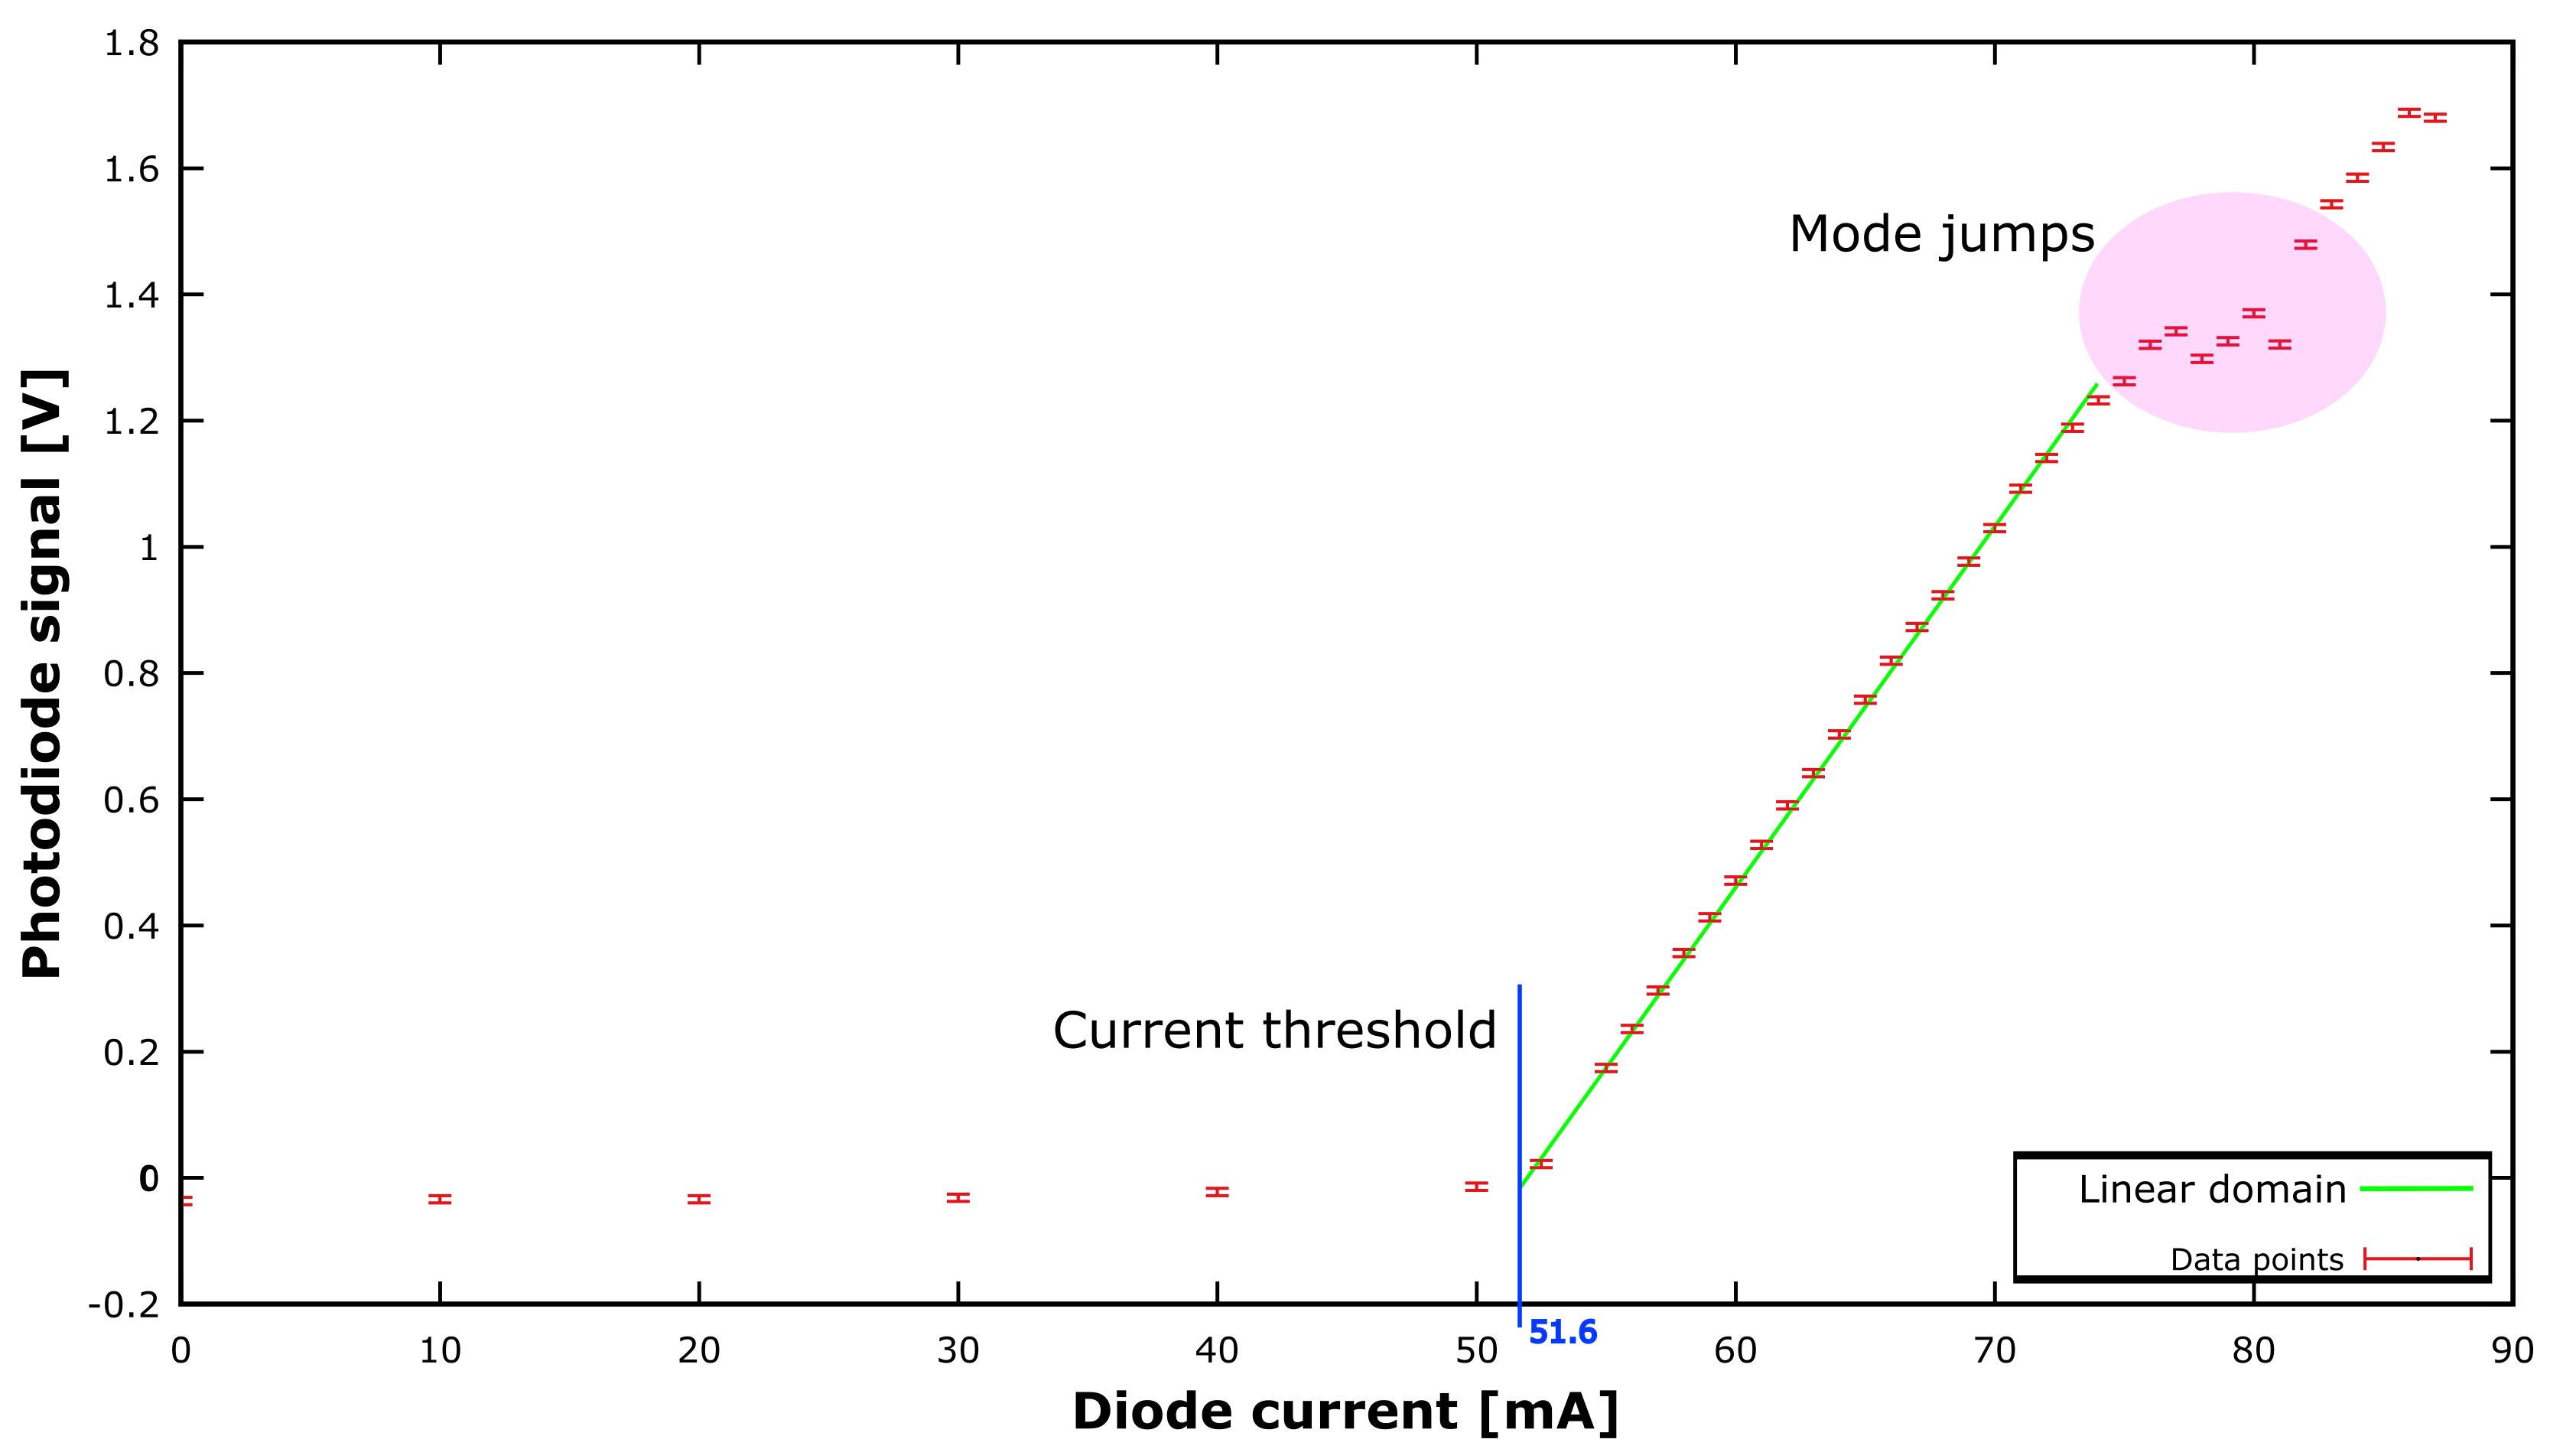
\includegraphics[width=1.0\linewidth]{graphics/characterization}
\caption[Characteristic curve of the laser diode]{The characteristic curve of the laser diode for supply currents up to $\unit{90}{mA}$. A mode jump can clearly be seen in the uper right corner.}
\label{fig:characterization}
\end{figure}


\subsection{Energy calibration}
\begin{figure}[htb]
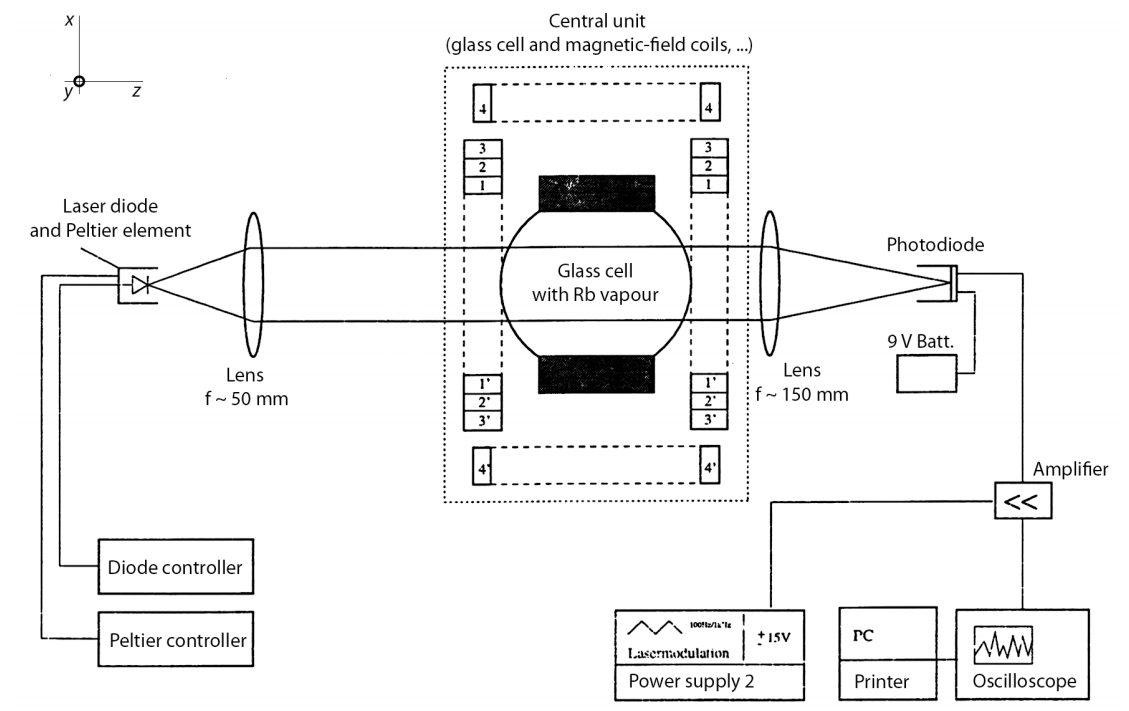
\includegraphics[width=1.0\linewidth]{graphics/generalsetup}
\caption[Experimental set-up for the Calibration]{Experimental set-up for the calibration measurements. An Ethalon is placed after the left lens.\cite{anleitung}}
\label{fig:calibration setup}
\end{figure}
A Fabry-Pérot-Interferometer (Ethalon), which is a set of parallel, almost completely reflecting surfaces facing each other, is used to gauge the diode. The intensity at the photo diode will be drastically dampened unless the laser wavelength allows for constructive interference to occur between the surfaces. The wavelengths at which light passes the interferometer are thus equidistant.When modulating the current through the diode by applying a saw-tooth voltage, the resulting intensity picture will ideally show perfectly equidistant peaks and thus allow for a calibration of the diode.\\

The diode current is then modified with a saw-tooth voltage, which is also used to trigger the oscilloscope(see figure \ref{fig:calibration setup}). 

